\chapter{Sistema de Tickets para soporte técnico}
Como parte de los ajustes  que se está realizando al clúster se encuentra la implementación de un sistema de Tickets para poder reportar problemas  de software, solicitar bibliotecas o  herramientas especiales a la administración del clúster. Luego de revisar las diferentes opciones disponibles, se ha optado por instalar el plugin JS Support Ticket  \cite{pluginTicket} utilizando Wordpress como plataforma. También se indica una alternativa instalando OSTicket más adelante. 

\section{Instalación de JS Support Ticket Plugin para Wordpress}
El proceso de instalación es similar al del plugin wpdirauth para integrar el LDAP. Iniciamos sesión como root y hacemos lo siguiente:
%%%%%%%%%%%%%%%%%%%%%%%%%%%%%%%%%%%%%%%%%%%%%%%%%%%%%%%%%%%%%%%%%%%%
\begin{lstlisting} 
wget https://downloads.wordpress.org/plugin/js-support-Ticket.1.1.7.zip
unzip  js-support-Ticket.1.1.7.zip
mv js-support-Ticket /var/www/html/wordpress/wp-content/plugins/
chmod -R +w /var/www/html/wordpress/wp-content/plugins/js-support-Ticket/
\end{lstlisting}
%%%%%%%%%%%%%%%%%%%%%%%%%%%%%%%%%%%%%%%%%%%%%%%%%%%%%%%%%%%%%%%%%%%%
En este caso,  damos permisos de escritura para  facilitar algunos ajustes de configuración. No se recomienda dejar esto siempre en este estado, por lo que al terminar de configurar todo, se recomienda eliminar estos permisos de escritura al menos para other.
%%%%%%%%%%%%%%%%%%%%%%%%%%%%%%%%%%%%%%%%%%%%%%%%%%%%%%%%%%%%%%%%%%%%
\begin{lstlisting} 
chmod -R o-w /var/www/html/wordpress/wp-content/plugins/js-support-Ticket/
\end{lstlisting}
%%%%%%%%%%%%%%%%%%%%%%%%%%%%%%%%%%%%%%%%%%%%%%%%%%%%%%%%%%%%%%%%%%%%
Una vez hecho lo anterior, ingresamos a la página del WordPress del clúster \url{http://cluster.cenat.ac.cr/wordpress/wp-admin/}. Debería aparecernos un prompt como el de la figura \ref{fig:js:01}.
%%%%%%%%%%%%%%%%%%%%%%%%%%%%%%%%%%%%%%%%%%%%%%%%%%%%%%%%%%%%%%%%%%%%
\begin{figure}[H]
\centering
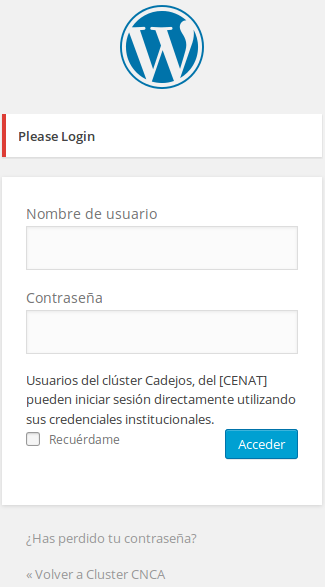
\includegraphics[width=0.35\textwidth]{ldap_plugin_settings03.png}
\caption{Pantalla de inicio de sesión.}
\label{fig:js:01}
\end{figure}
%%%%%%%%%%%%%%%%%%%%%%%%%%%%%%%%%%%%%%%%%%%%%%%%%%%%%%%%%%%%%%%%%%%%
Ahora procedemos a activar  el  plugin, de la misma  forma, nos dirigimos al menú Plugins y hacemos clic en el botón Activar por debajo del plugin JS-Support Ticket recién agregado. Debería verse de forma similar a como se muestra en la figura \ref{fig:js:02}.
%%%%%%%%%%%%%%%%%%%%%%%%%%%%%%%%%%%%%%%%%%%%%%%%%%%%%%%%%%%%%%%%%%%%
\begin{figure}[H]
\centering
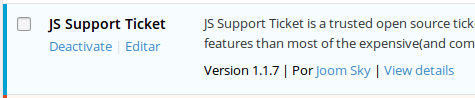
\includegraphics[width=0.35\textwidth]{js_plugin_activate.png}
\caption{Plugin para Tickets activado.}
\label{fig:js:02}
\end{figure}
%%%%%%%%%%%%%%%%%%%%%%%%%%%%%%%%%%%%%%%%%%%%%%%%%%%%%%%%%%%%%%%%%%%%
\section{Configuración general del plugin}
El menú del plugin debería aparecer al lado izquierdo. Ingresamos a este y luego hacemos clic en Configuraciones. En la parte superior se observan los diferentes menús según el tipo de configuración que se desea realizar. En las figuras \ref{fig:js:03}, \ref{fig:js:04}, \ref{fig:js:05}, \ref{fig:js:06}, \ref{fig:js:07}, \ref{fig:js:08}, \ref{fig:js:09}, y \ref{fig:js:10} se muestra la configuración general del plugin.
%%%%%%%%%%%%%%%%%%%%%%%%%%%%%%%%%%%%%%%%%%%%%%%%%%%%%%%%%%%%%%%%%%%%
\begin{figure}[H]
\centering
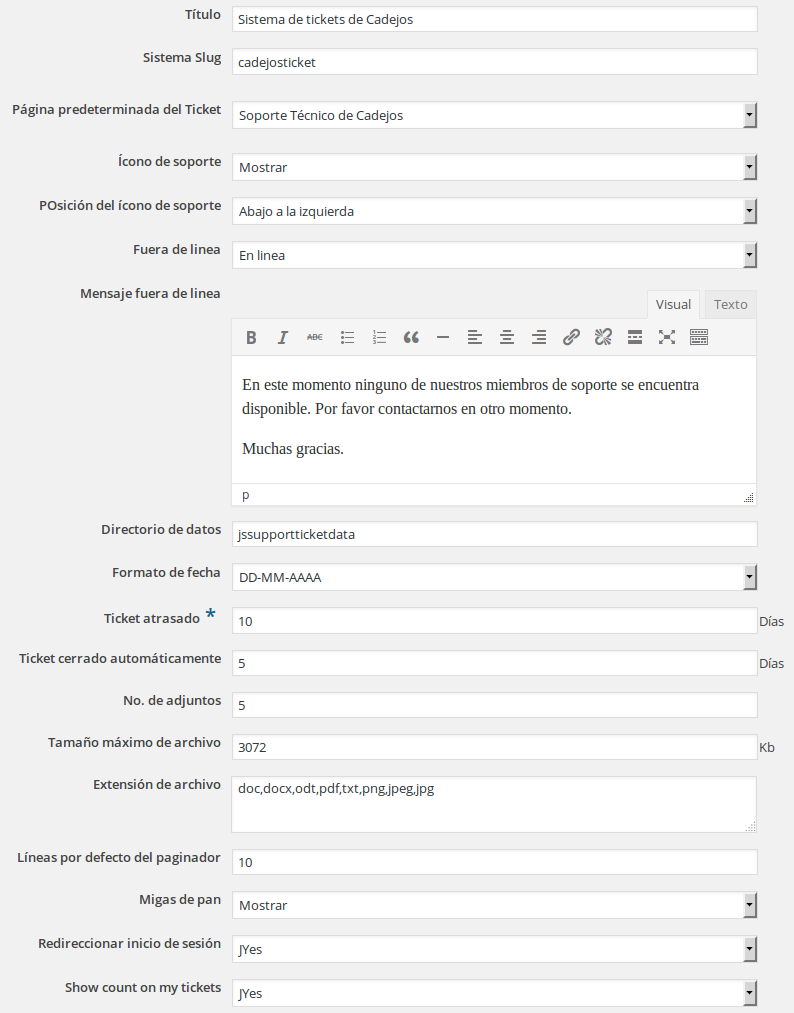
\includegraphics[width=0.5\textwidth]{js_plugin_settings00.png}
\caption{Ajustes generales del plugin.}
\label{fig:js:03}
\end{figure}
%%%%%%%%%%%%%%%%%%%%%%%%%%%%%%%%%%%%%%%%%%%%%%%%%%%%%%%%%%%%%%%%%%%%
\begin{figure}[H]
\centering
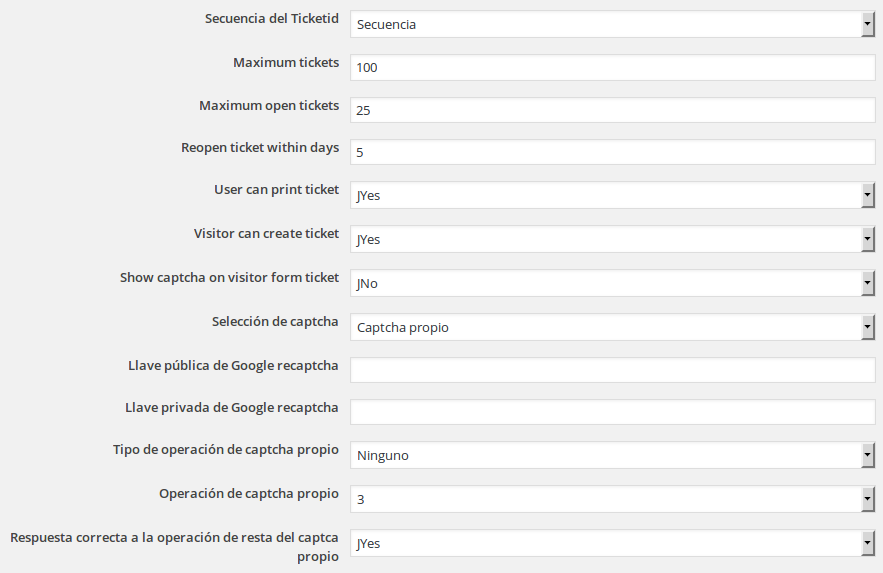
\includegraphics[width=0.5\textwidth]{js_plugin_settings01.png}
\caption{Configuración del Ticket.}
\label{fig:js:04}
\end{figure}
%%%%%%%%%%%%%%%%%%%%%%%%%%%%%%%%%%%%%%%%%%%%%%%%%%%%%%%%%%%%%%%%%%%%
\begin{figure}[H]
\centering
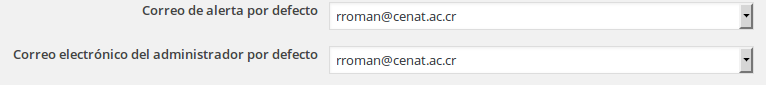
\includegraphics[width=0.5\textwidth]{js_plugin_settings02.png}
\caption{Correo de sistema por defecto.}
\label{fig:js:05}
\end{figure}
%%%%%%%%%%%%%%%%%%%%%%%%%%%%%%%%%%%%%%%%%%%%%%%%%%%%%%%%%%%%%%%%%%%%
\begin{figure}[H]
\centering
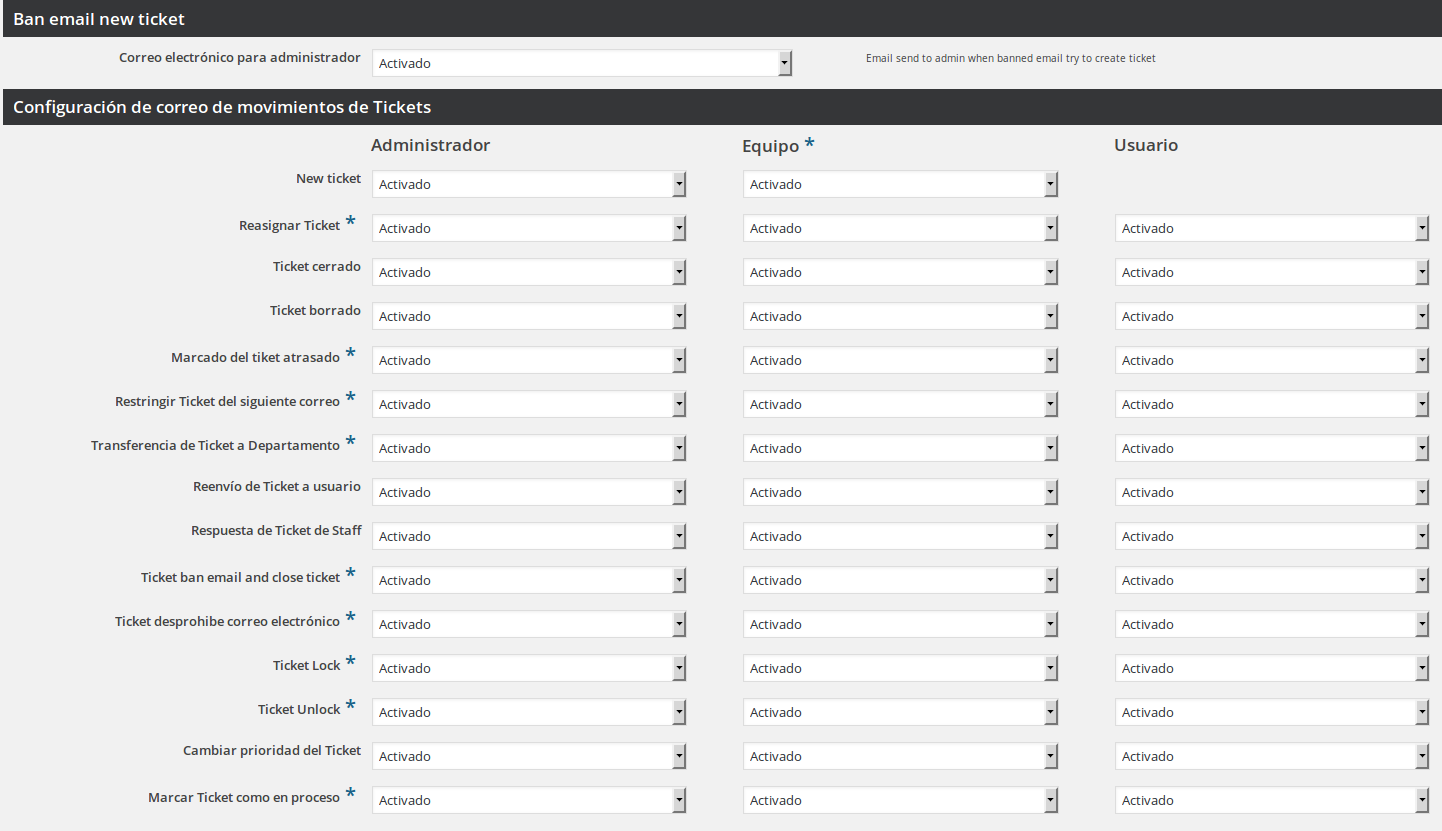
\includegraphics[width=0.5\textwidth]{js_plugin_settings03.png}
\caption{Configuración de correo de movimientos de Tickets.}
\label{fig:js:06}
\end{figure}
%%%%%%%%%%%%%%%%%%%%%%%%%%%%%%%%%%%%%%%%%%%%%%%%%%%%%%%%%%%%%%%%%%%%
\begin{figure}[H]
\centering
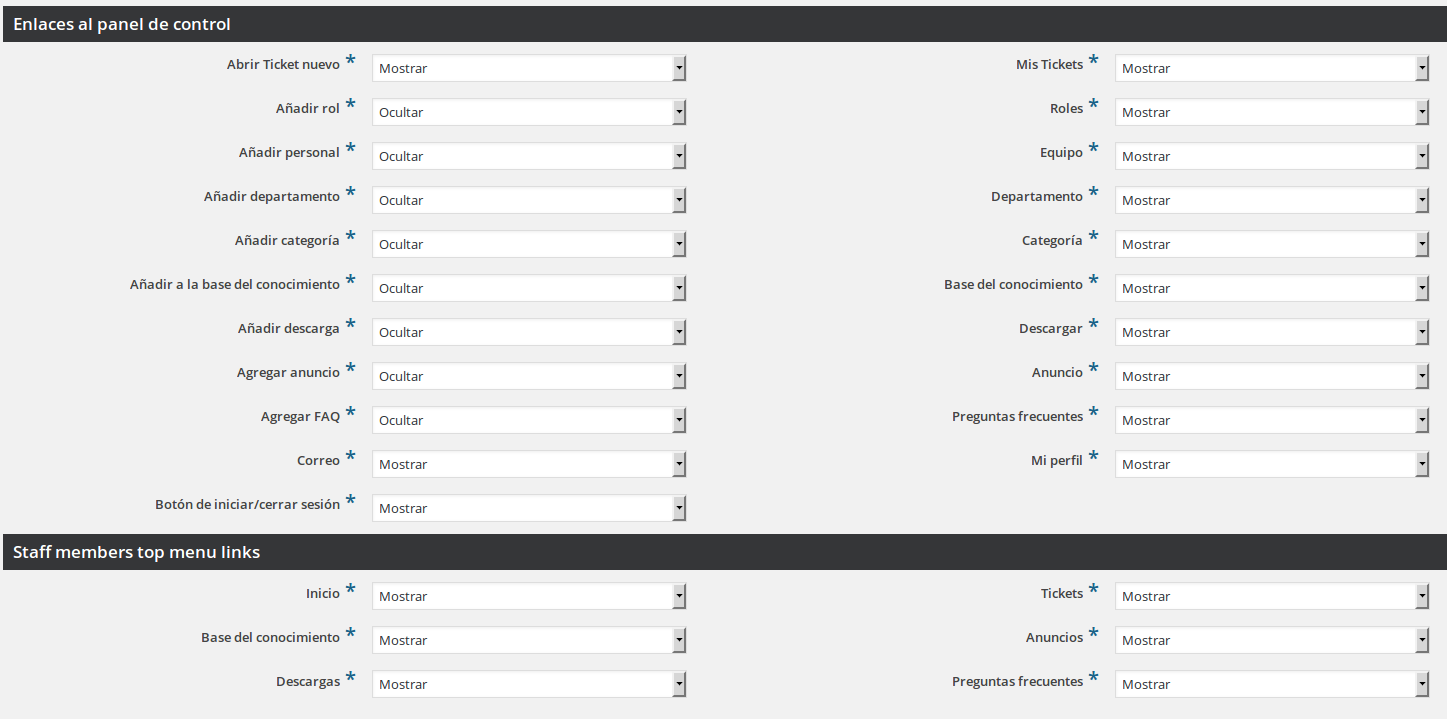
\includegraphics[width=0.5\textwidth]{js_plugin_settings04.png}
\caption{Ajustes del equipo de soporte.}
\label{fig:js:07}
\end{figure}
%%%%%%%%%%%%%%%%%%%%%%%%%%%%%%%%%%%%%%%%%%%%%%%%%%%%%%%%%%%%%%%%%%%%
\begin{figure}[H]
\centering
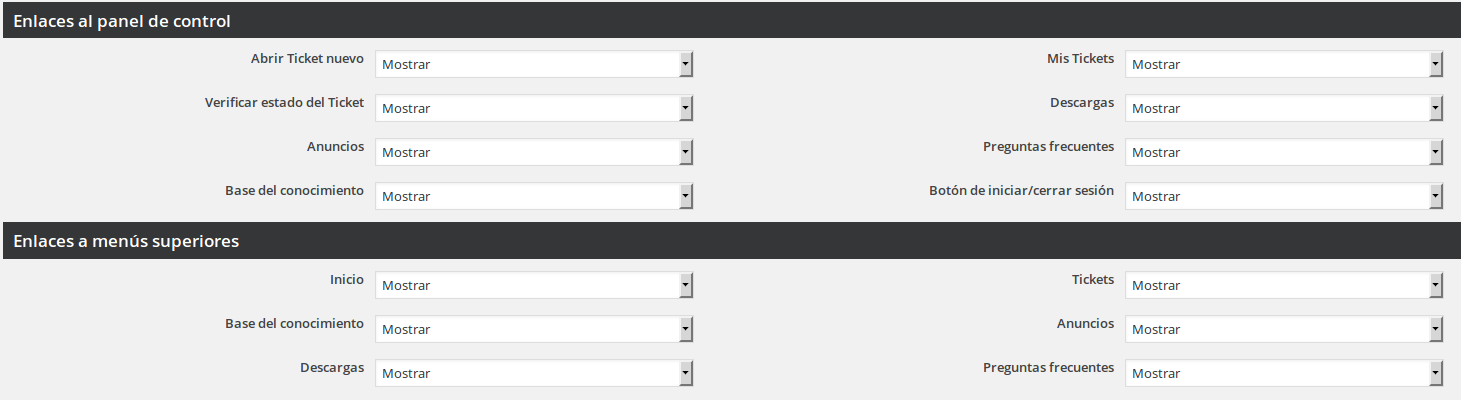
\includegraphics[width=0.5\textwidth]{js_plugin_settings05.png}
\caption{Ajustes del menú de usuario.}
\label{fig:js:08}
\end{figure}
%%%%%%%%%%%%%%%%%%%%%%%%%%%%%%%%%%%%%%%%%%%%%%%%%%%%%%%%%%%%%%%%%%%%
\begin{figure}[H]
\centering
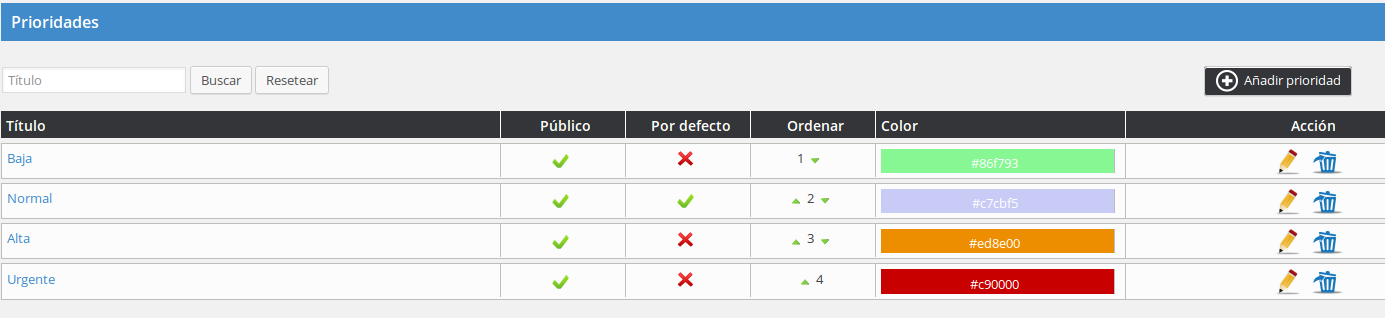
\includegraphics[width=0.5\textwidth]{js_plugin_settings06.png}
\caption{Ajustes de prioridad de Ticket.}
\label{fig:js:09}
\end{figure}
%%%%%%%%%%%%%%%%%%%%%%%%%%%%%%%%%%%%%%%%%%%%%%%%%%%%%%%%%%%%%%%%%%%%%%%%%
\begin{figure}[H]
\centering
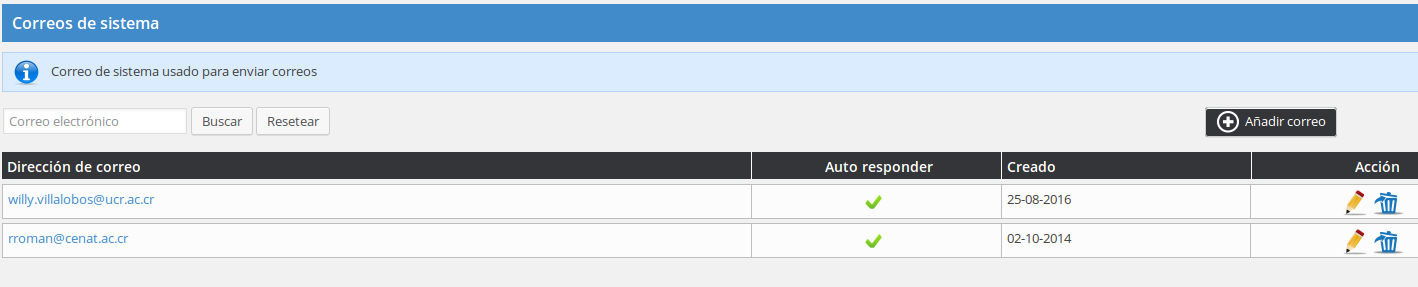
\includegraphics[width=0.5\textwidth]{js_plugin_settings07.png}
\caption{Direcciones de correo de soporte.}
\label{fig:js:10}
\end{figure}
%%%%%%%%%%%%%%%%%%%%%%%%%%%%%%%%%%%%%%%%%%%%%%%%%%%%%%%%%%%%%%%%%%%%%%%%%
\section{Plantillas de correo electrónico}
Dada la forma en la cual funciona  un sistema de Tickets generalmente, es natural considerar que existan respuestas predeterminadas para ciertos casos comunes, los cuales son enviados por correo electrónico tanto a usuarios como a administradores. En las figuras \ref{fig:js:11}, \ref{fig:js:12}, \ref{fig:js:13}, \ref{fig:js:14}, \ref{fig:js:15}, \ref{fig:js:16}, y \ref{fig:js:17} se muestran las plantillas de respuestas de correo electrónico implementadas en el sistema de Tickets de Cadejos. Los valores entre paréntesis cuadrados son variables que se pueden ajustar en cada caso.
%%%%%%%%%%%%%%%%%%%%%%%%%%%%%%%%%%%%%%%%%%%%%%%%%%%%%%%%%%%%%%%%%%%%%%%%%
\begin{figure}[H]
\centering
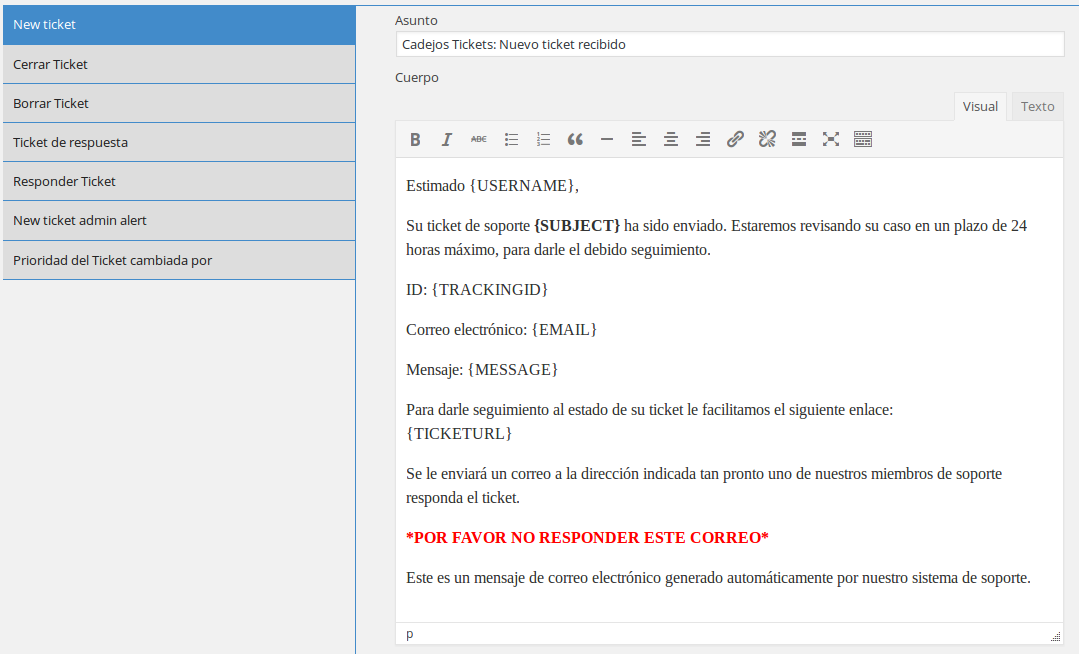
\includegraphics[width=0.5\textwidth]{js_plugin_mail00.png}
\caption{Plantilla para nuevo Ticket.}
\label{fig:js:11}
\end{figure}
%%%%%%%%%%%%%%%%%%%%%%%%%%%%%%%%%%%%%%%%%%%%%%%%%%%%%%%%%%%%%%%%%%%%%%%%%
\begin{figure}[H]
\centering
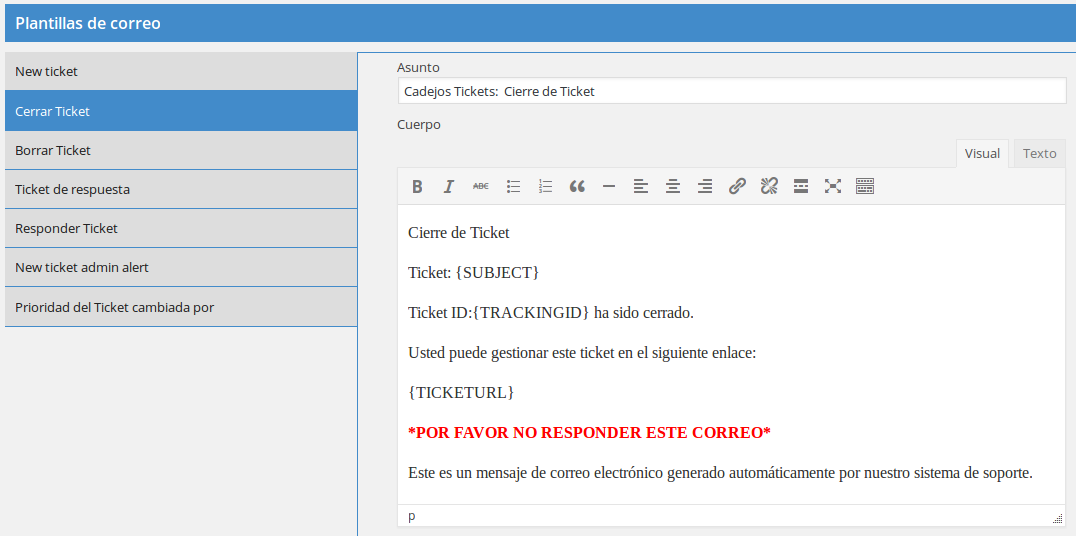
\includegraphics[width=0.5\textwidth]{js_plugin_mail01.png}
\caption{Plantilla para cierre de Ticket.}
\label{fig:js:12}
\end{figure}
%%%%%%%%%%%%%%%%%%%%%%%%%%%%%%%%%%%%%%%%%%%%%%%%%%%%%%%%%%%%%%%%%%%%%%%%%
\begin{figure}[H]
\centering
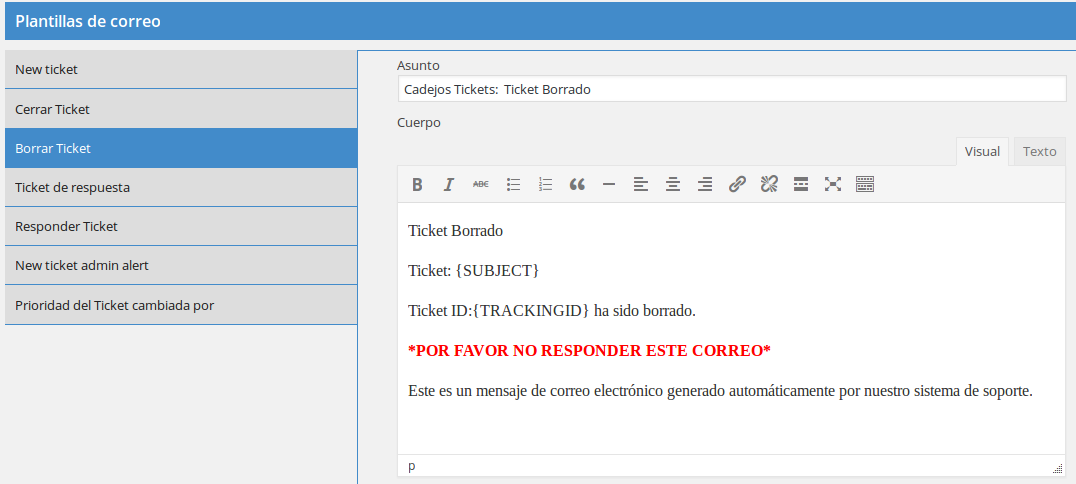
\includegraphics[width=0.5\textwidth]{js_plugin_mail02.png}
\caption{Plantilla para Ticket borrado.}
\label{fig:js:13}
\end{figure}
%%%%%%%%%%%%%%%%%%%%%%%%%%%%%%%%%%%%%%%%%%%%%%%%%%%%%%%%%%%%%%%%%%%%%%%%%
\begin{figure}[H]
\centering
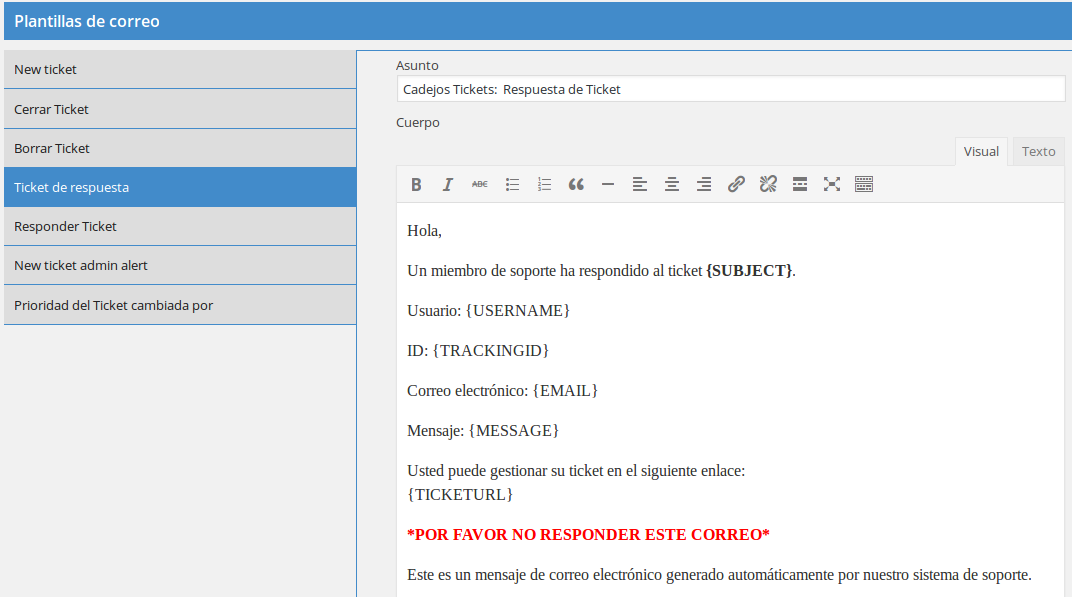
\includegraphics[width=0.5\textwidth]{js_plugin_mail03.png}
\caption{Plantilla para respuesta de un administrador a un Ticket.}
\label{fig:js:14}
\end{figure}
%%%%%%%%%%%%%%%%%%%%%%%%%%%%%%%%%%%%%%%%%%%%%%%%%%%%%%%%%%%%%%%%%%%%%%%%%
\begin{figure}[H]
\centering
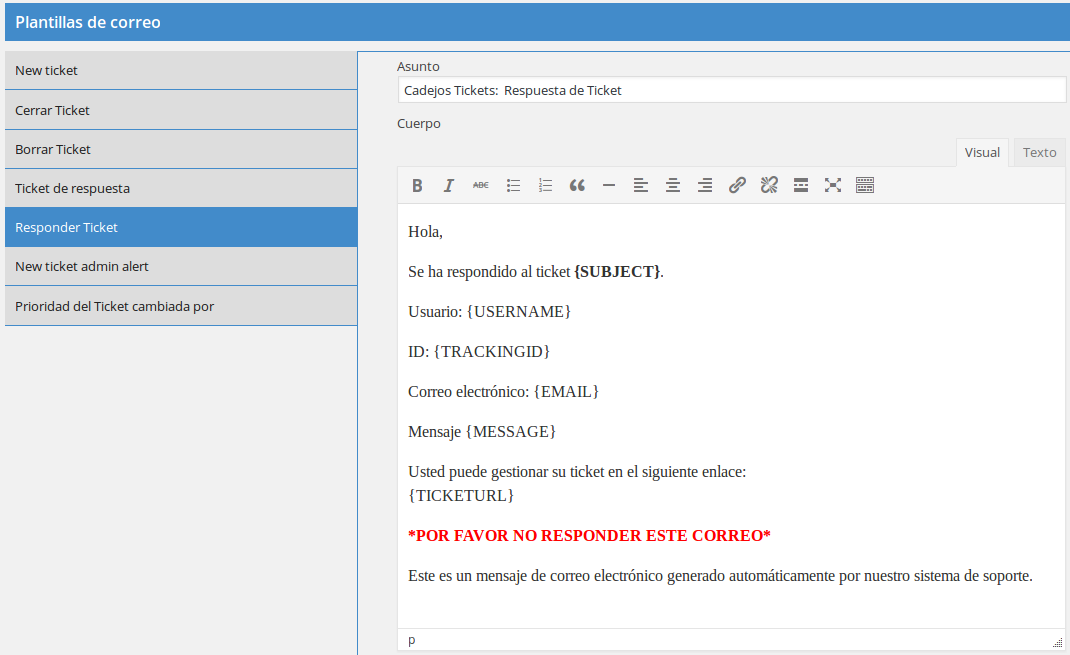
\includegraphics[width=0.5\textwidth]{js_plugin_mail04.png}
\caption{Plantilla de respuesta  genérica a un Ticket.}
\label{fig:js:15}
\end{figure}
%%%%%%%%%%%%%%%%%%%%%%%%%%%%%%%%%%%%%%%%%%%%%%%%%%%%%%%%%%%%%%%%%%%%%%%%%
\begin{figure}[H]
\centering
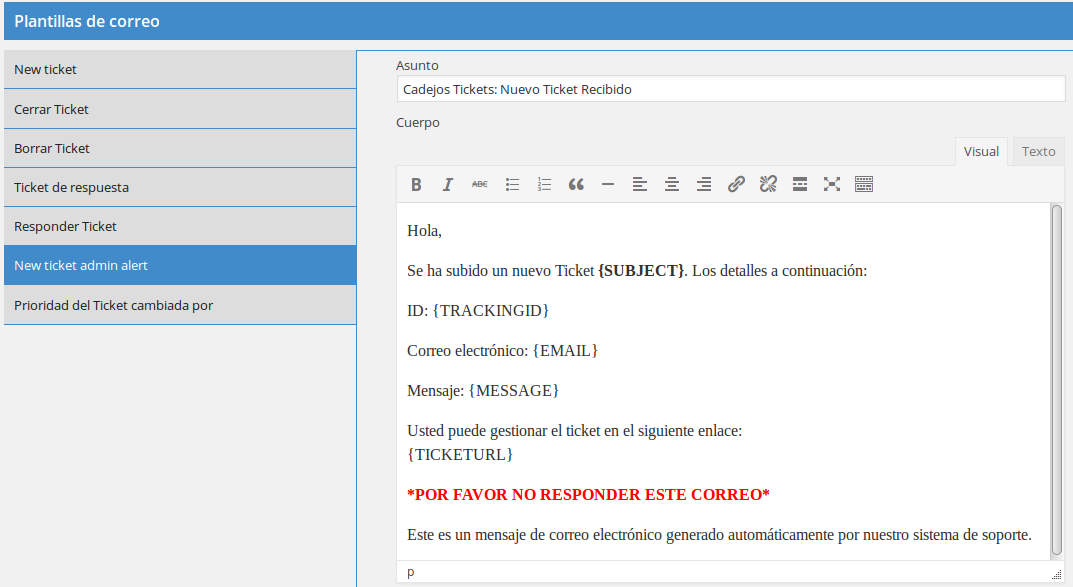
\includegraphics[width=0.5\textwidth]{js_plugin_mail05.png}
\caption{Plantilla de alerta de Ticket para el administrador.}
\label{fig:js:16}
\end{figure}
%%%%%%%%%%%%%%%%%%%%%%%%%%%%%%%%%%%%%%%%%%%%%%%%%%%%%%%%%%%%%%%%%%%%%%%%%
\begin{figure}[H]
\centering
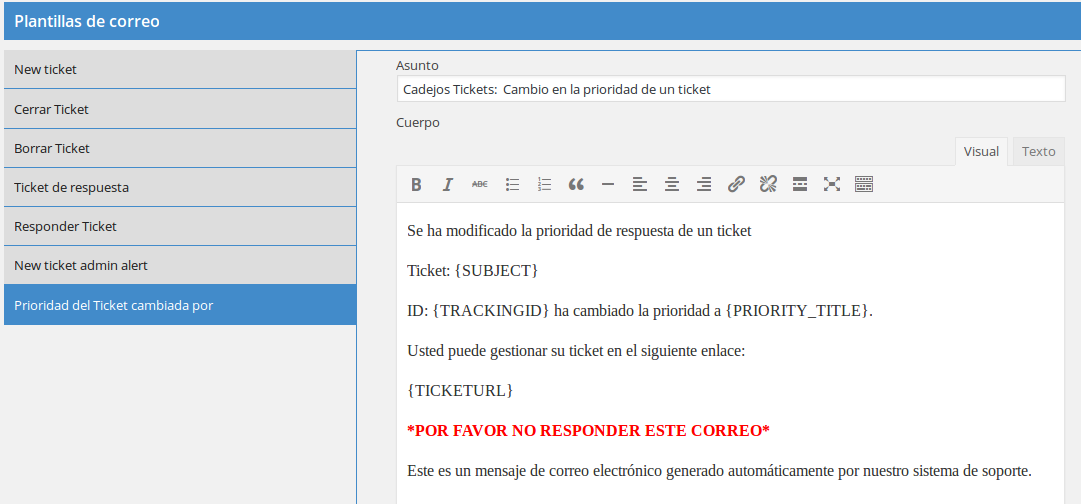
\includegraphics[width=0.5\textwidth]{js_plugin_mail06.png}
\caption{Plantlla de cambio de prioridad en el Ticket enviado.}
\label{fig:js:17}
\end{figure}
%%%%%%%%%%%%%%%%%%%%%%%%%%%%%%%%%%%%%%%%%%%%%%%%%%%%%%%%%%%%%%%%%%%%%%%%%
\section{Traducción del plugin al idioma Español}
Como se ha podido observar en algunas secciones de la interfaz de configuración y de uso del sistema de Tickets, hay títulos y rótulos que aparecen en inglés o están mal traducidas. Este tipo de detalles generalmente es posible corregirlos con tan solo instalar el  plugin en el idioma deseado, sin embargo, en este caso el proyecto de traducción es un esfuerzo independiente. Dada la necesidad de mantener cierta homogeneidad en el plugin en cuanto al idioma, se requiere modificar las plantillas de traducción disponibles. Estas se pueden descargar en el enlace \url{http://www.joomsky.com/translations.html}, donde se indican además las instrucciones a seguir para poder instalar el idioma, tal y como se muestra en la figura \ref{fig:js:18}
%%%%%%%%%%%%%%%%%%%%%%%%%%%%%%%%%%%%%%%%%%%%%%%%%%%%%%%%%%%%%%%%%%%%%%%%%
\begin{figure}[H]
\centering
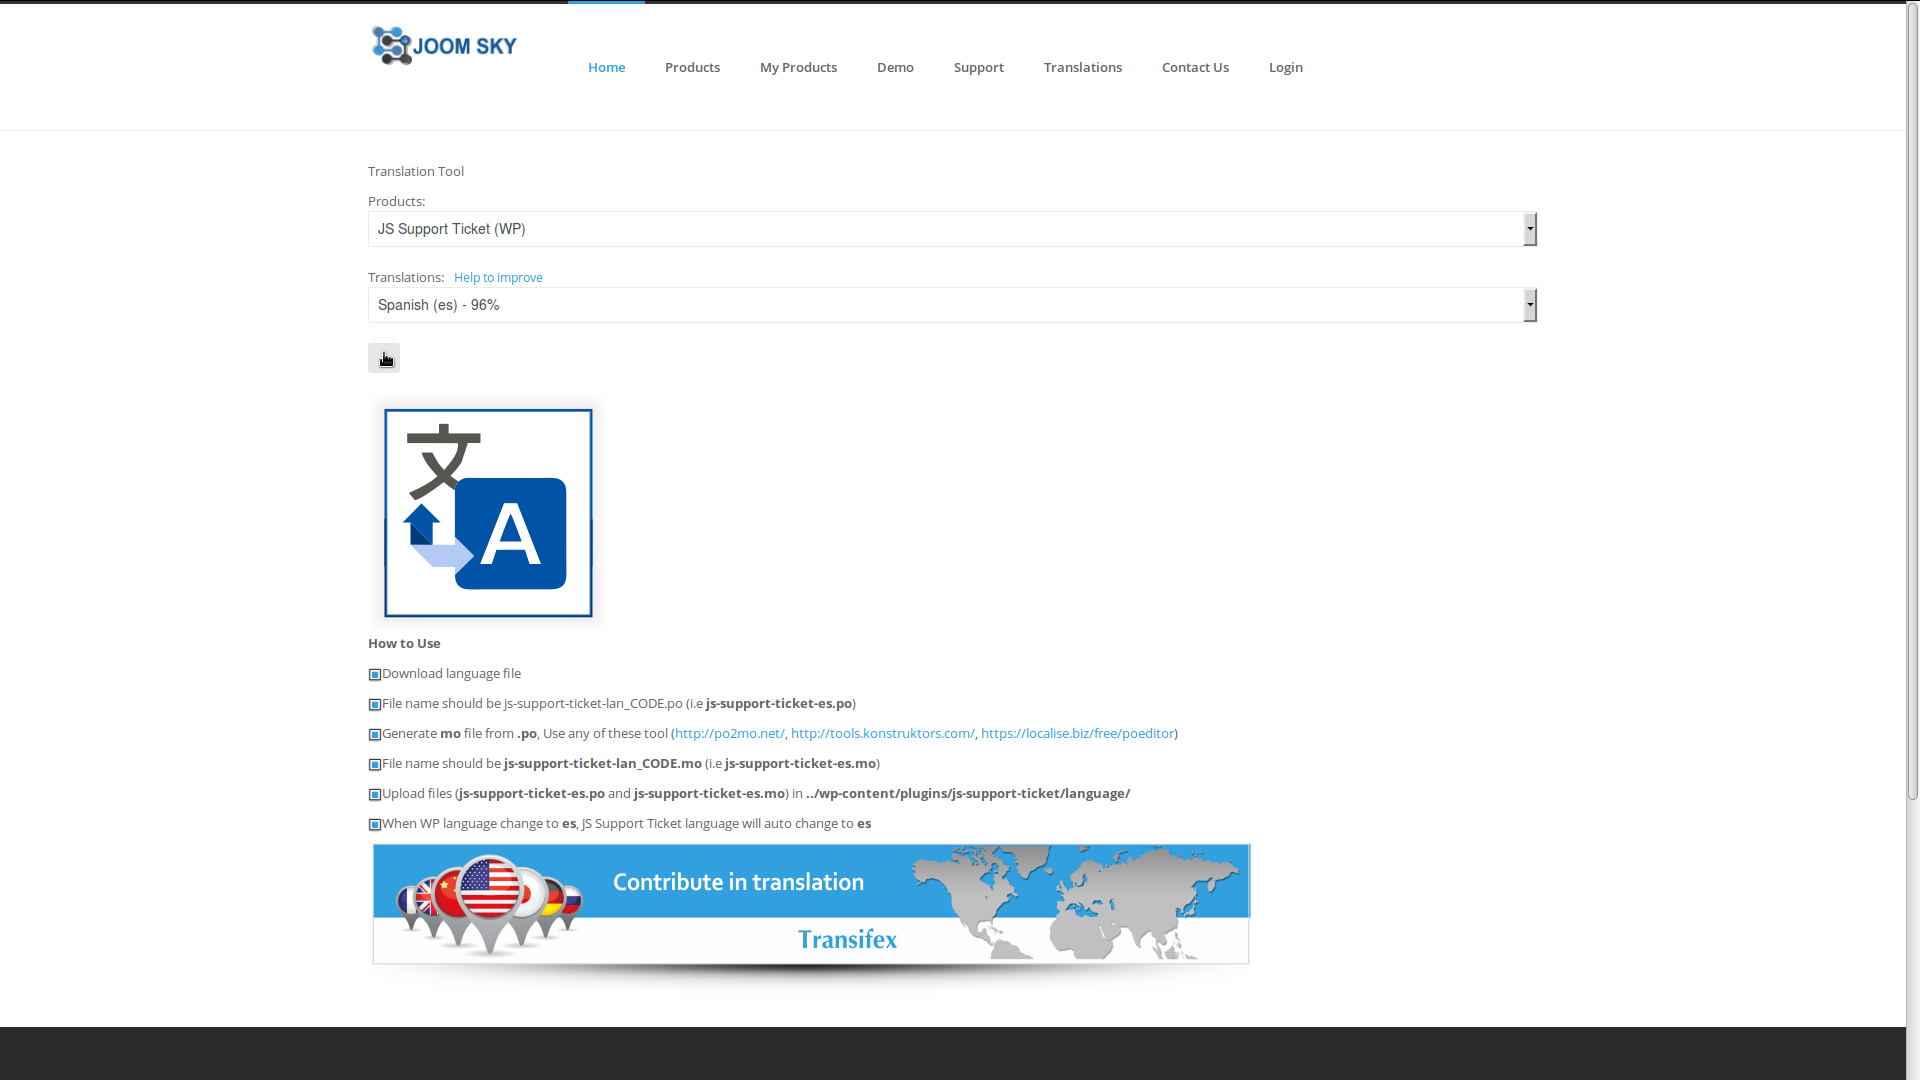
\includegraphics[width=0.5\textwidth]{js_lang00.png}
\caption{Sitio para descargar el paquete de idiomas para el sistema de Tickets.}
\label{fig:js:18}
\end{figure}
%%%%%%%%%%%%%%%%%%%%%%%%%%%%%%%%%%%%%%%%%%%%%%%%%%%%%%%%%%%%%%%%%%%%%%%%%
Si se desea modificar el archivo de idioma para corregir errores o agregar nuevas oraciones, frases o etiquetas para traducir, se debe modificar el archivo.po  con cualquier editor de texto. Posterior a eso se debe generar el archivo homólogo archivo.mo. Para esto se debe visitar el sitio \url{http://po2mo.net/}, subir el archivo.po y hacer clic en Convert, como se muestra en la figura \ref{fig:js:19}. Posteriormente se descarga el archivo.mo generado, procurando que ambos tengan el mismo nombre, y se copian al directorio /var/www/html/wordpress/wp-content/plugins/js-support-Ticket/languages/ en Cadejos.
%%%%%%%%%%%%%%%%%%%%%%%%%%%%%%%%%%%%%%%%%%%%%%%%%%%%%%%%%%%%%%%%%%%%%%%%%

\begin{figure}[H]
\centering
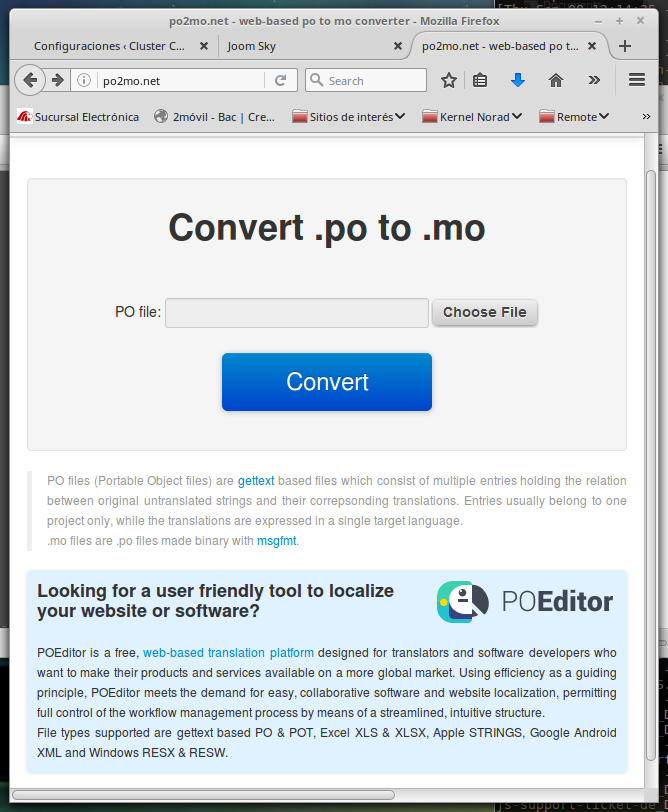
\includegraphics[width=0.5\textwidth]{js_lang01.png}
\caption{Sitio para convertir la plantilla de traducción a formato .mo.}
\label{fig:js:19}
\end{figure}

%%%%%%%%%%%%%%%%%%%%%%%%%%%%%%%%%%%%%%%%%%%%%%%%%%%%%%%%%%%%%%%%%%%%%%%%%
De forma alternativa, es posible realizar esta conversión de archivos desde la terminal, utilizando el programa gettext \cite{mo2po}. Inicialmente corroboramos si está instalado, de otro modo lo instalamos.
%%%%%%%%%%%%%%%%%%%%%%%%%%%%%%%%%%%%%%%%%%%%%%%%%%%%%%%%%%%%%%%%%%%%%%%%%
\begin{lstlisting} 
yum install gettext
\end{lstlisting}
%%%%%%%%%%%%%%%%%%%%%%%%%%%%%%%%%%%%%%%%%%%%%%%%%%%%%%%%%%%%%%%%%%%%%%%%%
Este programa permite la conversión tanto de archivos.po a .mo y viceversa, por lo que resulta de gran utilidad cuando no se dispone de uno u otro a la hora de traducir plugins de WordPress u otra aplicación. Su uso es bastante simple:
%%%%%%%%%%%%%%%%%%%%%%%%%%%%%%%%%%%%%%%%%%%%%%%%%%%%%%%%%%%%%%%%%%%%%%%%%
\begin{lstlisting} 
msgfmt file.po -o file.mo
msgunfmt file.mo -o file.po
\end{lstlisting}
%%%%%%%%%%%%%%%%%%%%%%%%%%%%%%%%%%%%%%%%%%%%%%%%%%%%%%%%%%%%%%%%%%%%%%%%%
A la hora de convertir a .mo el programa dará error cuando encuentre entradas duplicadas y otra serie de errores, siempre especificando las líneas problemáticas para que el usuario pueda arreglar el problema.
%%%%%%%%%%%%%%%%%%%%%%%%%%%%%%%%%%%%%%%%%%%%%%%%%%%%%%%%%%%%%%%%%%%%%%%%%
\begin{lstlisting} 
msgfmt js-support-Ticket-es_ES.po -o js-support-Ticket-es_ES.mo
js-support-Ticket-es_ES.po:405: duplicate message definition...
js-support-Ticket-es_ES.po:400: ...this is the location of the first definition
js-support-Ticket-es_ES.po:597: duplicate message definition...
js-support-Ticket-es_ES.po:592: ...this is the location of the first definition
msgfmt: found 2 fatal errors
\end{lstlisting}
%%%%%%%%%%%%%%%%%%%%%%%%%%%%%%%%%%%%%%%%%%%%%%%%%%%%%%%%%%%%%%%%%%%%%%%%%
\section{Modificaciones a la apariencia del plugin para afinar estética}
Dado que generalmente los plugins de WordPress  se hacen pensando particularmente en un público meta anglosajón, algunas traducciones comunitarias como la utilizada anteriormente generan errores en como se despliega la página final en el navegador, típicamente en la forma de textos que se salen de los cuadros. Es por ello que se recomienda hacer una inspección a fondo de toda la interfaz final del plugin. En caso de encontrar defectos en la visualización del plugin,  es posible aislar qué línea específica es la que da problemas utilizando la consola de javascript del navegador (para el caso de Firefox, se invoca presionando ctrl+shift+c). A continuación se muestra un ejemplo rápido de cómo emplear esta poderosa herramienta para depurar sitios. Al abrir un navegador y dirigirnos al sitio \url{cluster.cenat.ac.cr} y presionar ctrl+shift+c vemos una vista similar al de la figura \ref{fig:js:20}. La consola inferior se compone de una serie de opciones las cuales son, de izquierda a derecha: inspeccionar elemento, inspector,  consola, depurador, editor  de estilo, rendimiento, red, una barra de búsqueda de html, un botón para ocultar los elementos del css (para efectos de estilo), así como botones para aislar más efectivamente las líneas de código que permiten el despliegue de lo que se ve en la página cuando se ingresa.
%%%%%%%%%%%%%%%%%%%%%%%%%%%%%%%%%%%%%%%%%%%%%%%%%%%%%%%%%%%%%%%%%%%%%%%%%
\begin{figure}[H]
\centering
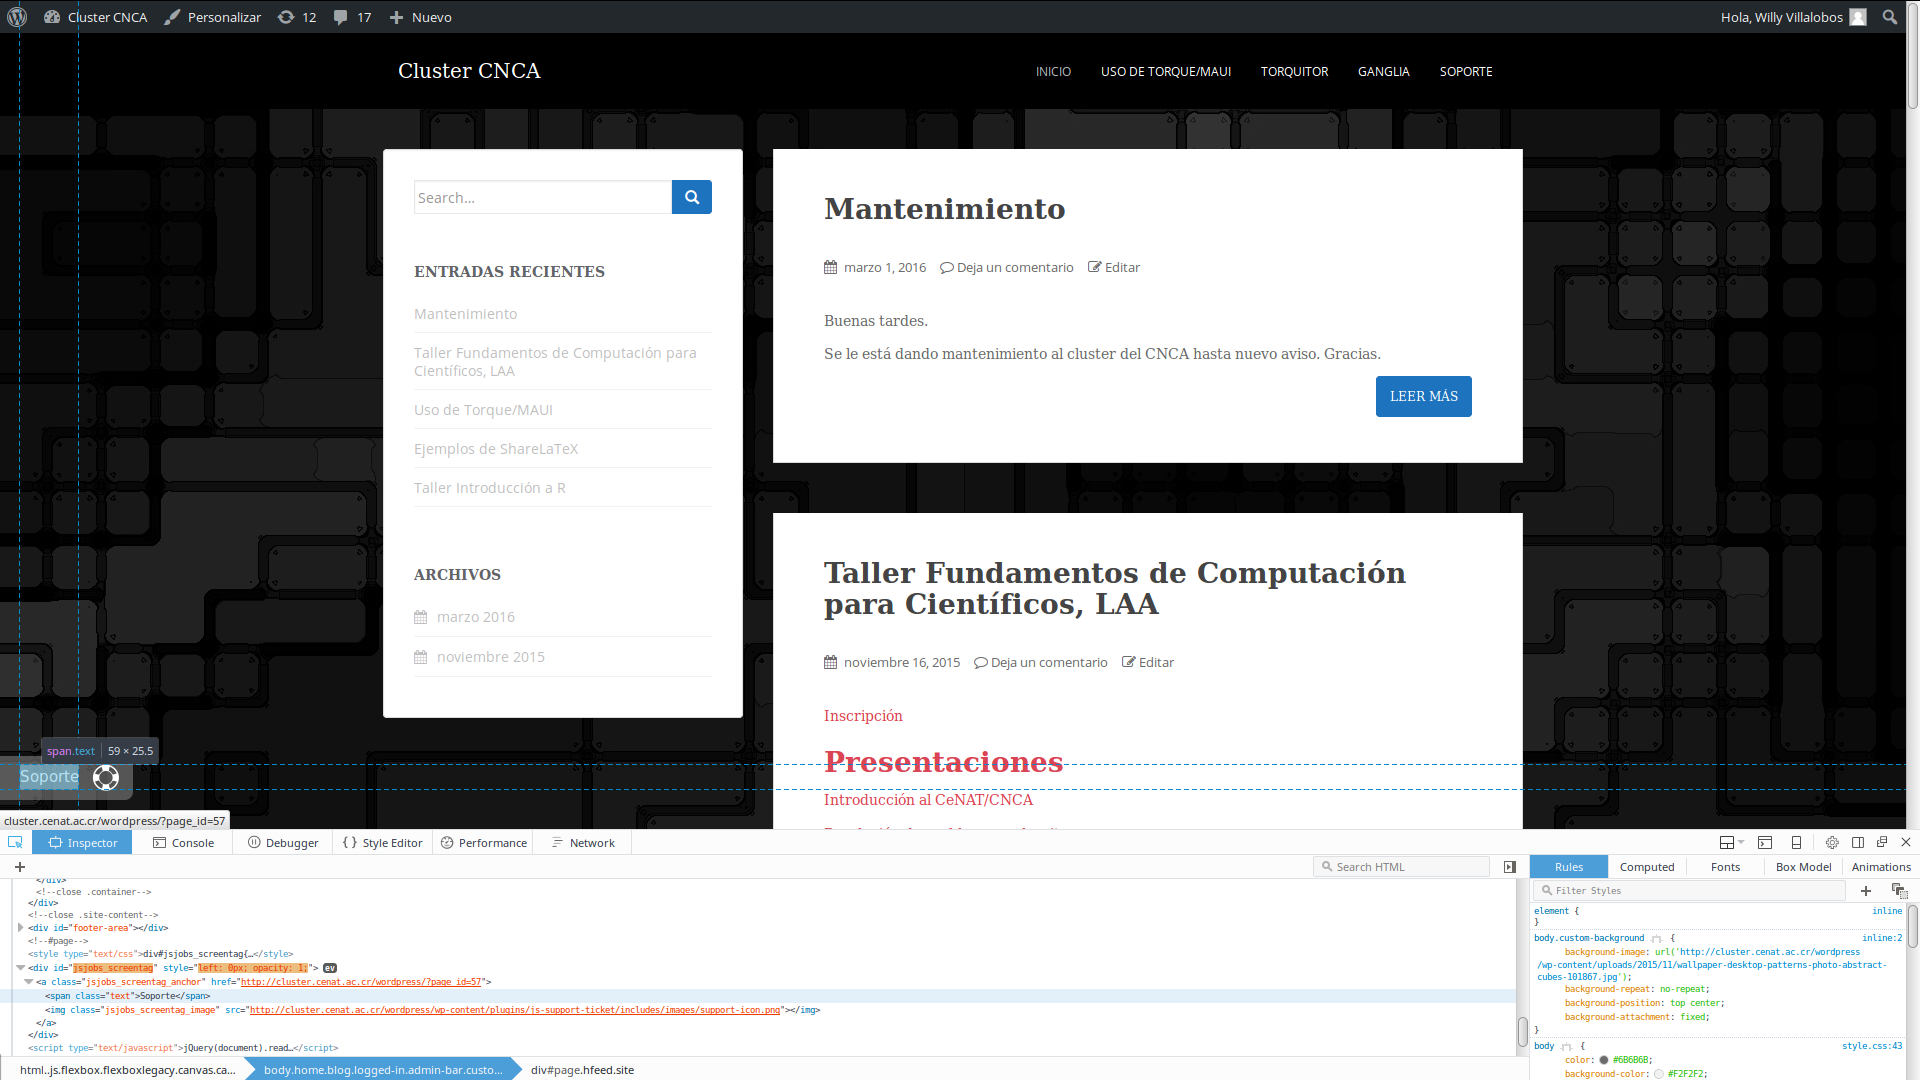
\includegraphics[width=0.5\textwidth]{webconsole00.png}
\caption{Consola para inspección de elementos de un sitio web.}
\label{fig:js:20}
\end{figure}
%%%%%%%%%%%%%%%%%%%%%%%%%%%%%%%%%%%%%%%%%%%%%%%%%%%%%%%%%%%%%%%%%%%%%%%%%
El  código desplegado abajo corresponde a los  archivos .php, .html y .css que generan la vista actual de la página. Si hay un elemento de interés  que deseamos inspeccionar, hacemos clic  sobre el botón de inspeccionar elemento y hacemos luego clic sobre el elemento de interés. Inmediatamente la  consola nos dirigirá a la línea de código de interés, y al lado derecho veremos las líneas del css que configuran el aspecto del elemento inspeccionado. Si hay algo en particular que deseamos corregir simplemente aislamos la línea de código y nos vamos a la consola para realizar una búsqueda del archivo que contiene esa línea para modificarla \cite{textinfile}.
%%%%%%%%%%%%%%%%%%%%%%%%%%%%%%%%%%%%%%%%%%%%%%%%%%%%%%%%%%%%%%%%%%%%%%%%%
\begin{lstlisting} 
grep -lir " texto que deseamos encontrar " /var/www/html/wordpress
\end{lstlisting}
%%%%%%%%%%%%%%%%%%%%%%%%%%%%%%%%%%%%%%%%%%%%%%%%%%%%%%%%%%%%%%%%%%%%%%%%%
Este comando los listará los archivos que contienen líneas idénticas a la proporcionada para poder proceder  a modificarlas si fuese necesario. De esta forma es posible manipular el aspecto de las páginas y los plugins que se instalan para poder presentar una mejor estética a los usuarios finales. Intentemos con un ejemplo. Considere la figura \ref{fig:js:21} donde se presenta un cuadro cuyo texto no encaja adecuadamente. si hacemos clic en inspeccionar elemento y luego clic en el botón que presenta el defecto visual como se muestra en la figura \ref{fig:js:22}, vemos cómo las consolas inferiores nos despliegan el código correspondiente a ese botón, tal y como se muestra en la figura \ref{fig:js:23}. Para este caso nos interesa corregir el tamaño de la fuente del bloque que dice "Contestado(0). La línea correspondiente es:
%%%%%%%%%%%%%%%%%%%%%%%%%%%%%%%%%%%%%%%%%%%%%%%%%%%%%%%%%%%%%%%%%%%%%%%%%
\begin{lstlisting}[language=php]
<a class="js-myTicket-link 
"href="http://cluster.cenat.ac.cr/wordpress/?page_id=57&amp;
jstmod=Ticket&amp;jstlay=myTicket&amp;list=3">
Contestado ( 0 )</a>
\end{lstlisting}
%%%%%%%%%%%%%%%%%%%%%%%%%%%%%%%%%%%%%%%%%%%%%%%%%%%%%%%%%%%%%%%%%%%%%%%%%
De forma similar, la línea que define el tamaño del teto en el cuadro se ubica en el archivo style.css en la linea 43, según se muestra en la figura \ref{fig:js:24}.
%%%%%%%%%%%%%%%%%%%%%%%%%%%%%%%%%%%%%%%%%%%%%%%%%%%%%%%%%%%%%%%%%%%%%%%%%
\begin{figure}[H]
\centering
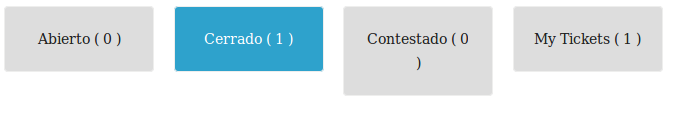
\includegraphics[width=0.5\textwidth]{webconsole01.png}
\caption{Cuadro de texto del plugin de JS Support Tickets a inspeccionar.}
\label{fig:js:21}
\end{figure}
%%%%%%%%%%%%%%%%%%%%%%%%%%%%%%%%%%%%%%%%%%%%%%%%%%%%%%%%%%%%%%%%%%%%%%%%%
\begin{figure}[H]
\centering
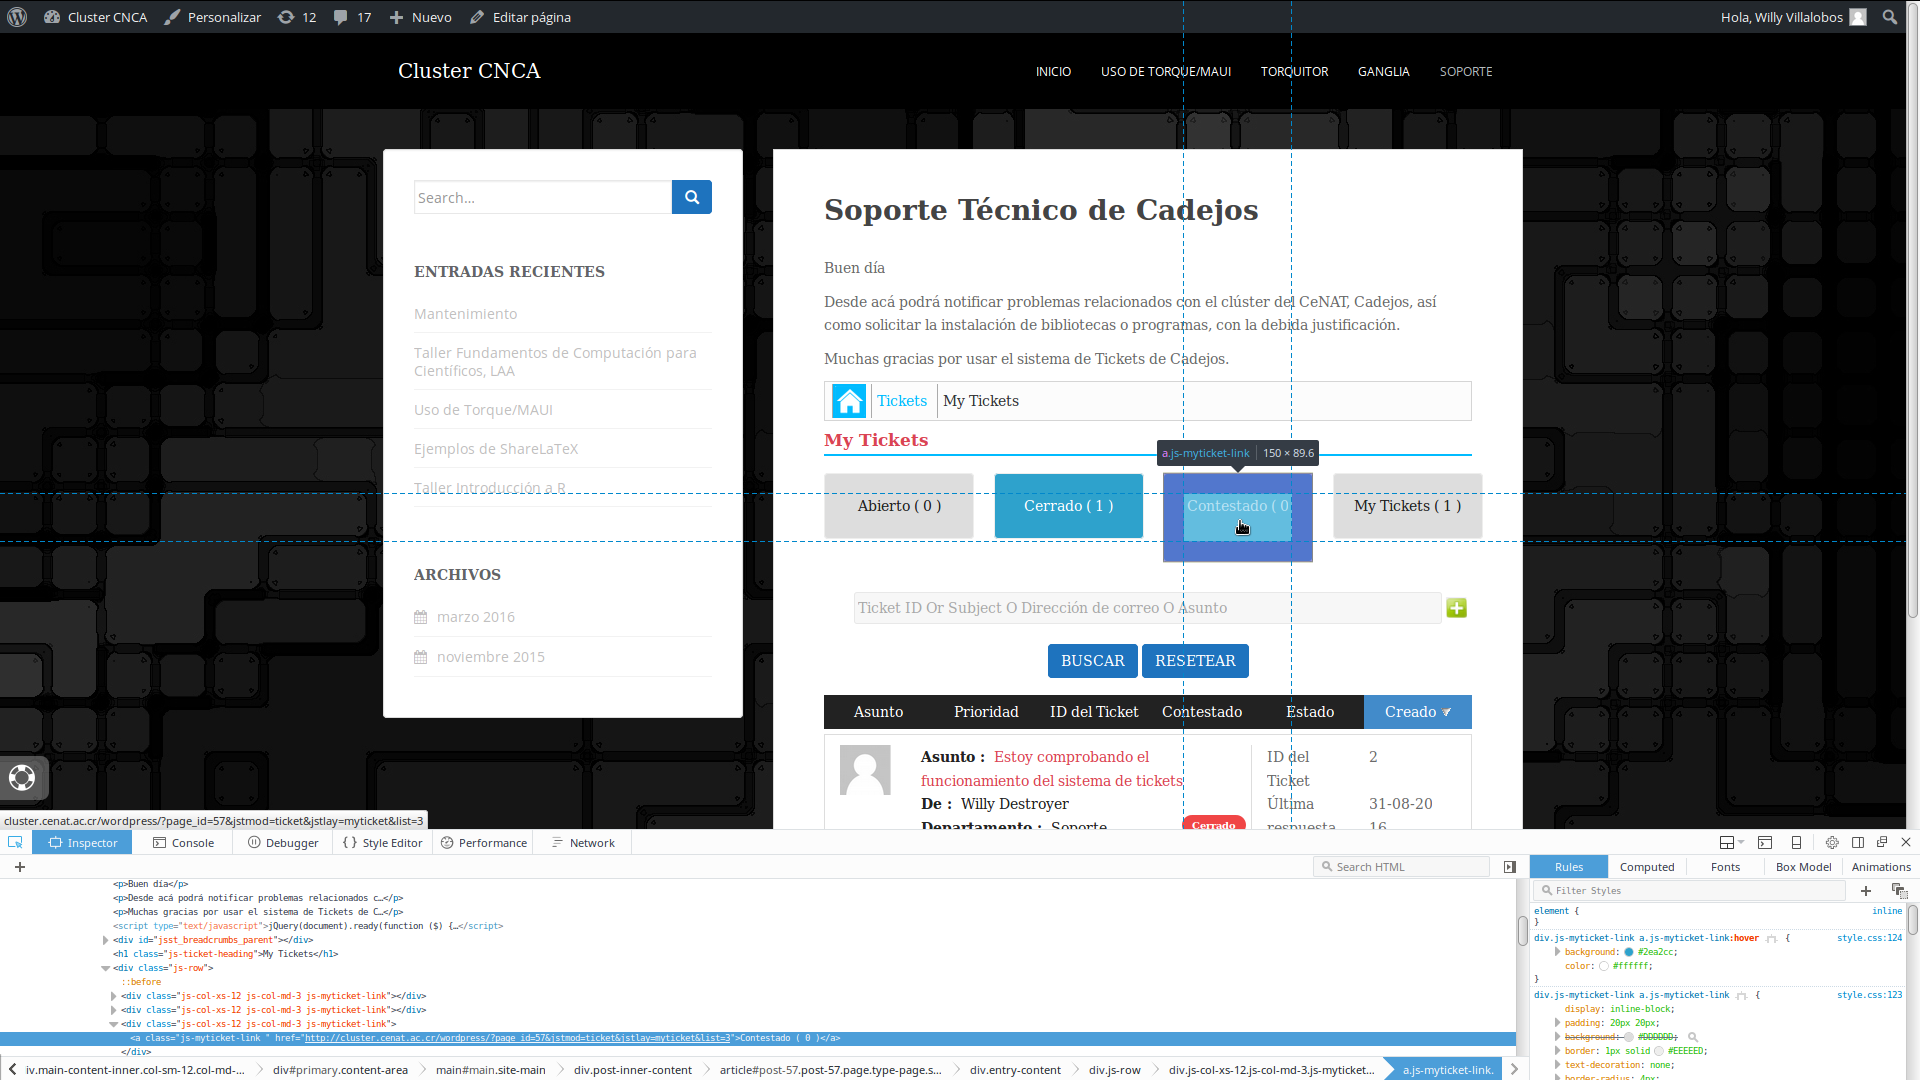
\includegraphics[width=0.5\textwidth]{webconsole02.png}
\caption{Inspección de elemento problemático.}
\label{fig:js:22}
\end{figure}
%%%%%%%%%%%%%%%%%%%%%%%%%%%%%%%%%%%%%%%%%%%%%%%%%%%%%%%%%%%%%%%%%%%%%%%%%
\begin{figure}[H]
\centering
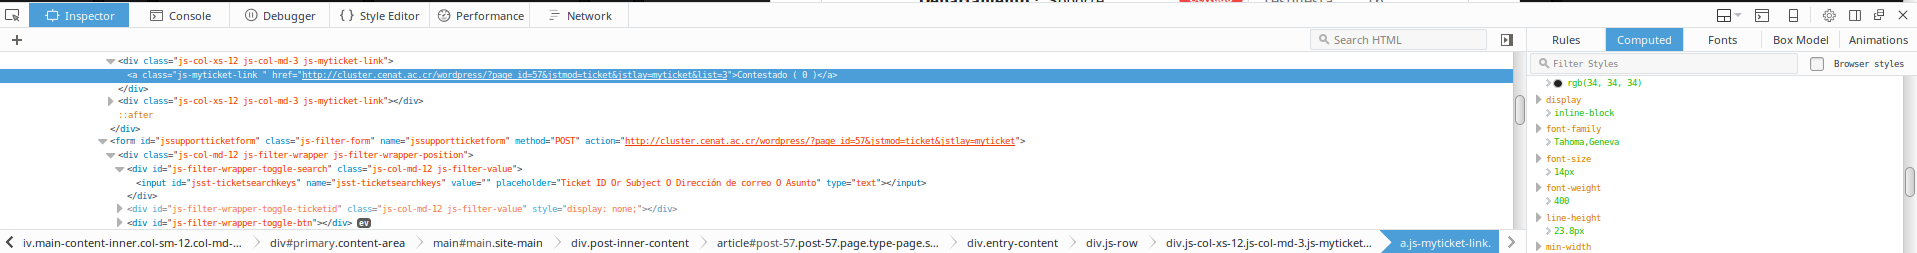
\includegraphics[width=0.5\textwidth]{webconsole03.png}
\caption{Código responsable del despliegue del botón.}
\label{fig:js:23}
\end{figure}
%%%%%%%%%%%%%%%%%%%%%%%%%%%%%%%%%%%%%%%%%%%%%%%%%%%%%%%%%%%%%%%%%%%%%%%%%
\begin{figure}[H]
\centering
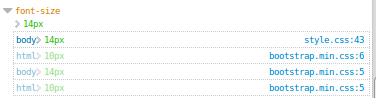
\includegraphics[width=0.5\textwidth]{webconsole04.png}
\caption{Segmento del css encargado del tamaño de la letra del  cuadro.}
\label{fig:js:24}
\end{figure}
%%%%%%%%%%%%%%%%%%%%%%%%%%%%%%%%%%%%%%%%%%%%%%%%%%%%%%%%%%%%%%%%%%%%%%%%%
Teniendo aislados estos elementos, podemos buscarlos usando el comando grep de la forma presentada anteriormente, así como usar el comando locate para encontrar el archivo style.css que se debe modificar si fuese necesario. El resultado final se muestra en la figura \ref{fig:js:25}, donde se ubicó la línea div.js-myTicket-link y se  agregó al final el tamaño explícito de la fuente font-size:14px;.
%%%%%%%%%%%%%%%%%%%%%%%%%%%%%%%%%%%%%%%%%%%%%%%%%%%%%%%%%%%%%%%%%%%%%%%%%
\begin{figure}[H]
\centering
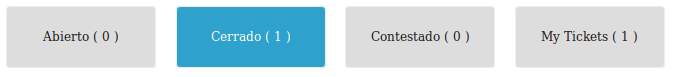
\includegraphics[width=0.5\textwidth]{webconsole05.png}
\caption{Botón corregido.}
\label{fig:js:25}
\end{figure}
%%%%%%%%%%%%%%%%%%%%%%%%%%%%%%%%%%%%%%%%%%%%%%%%%%%%%%%%%%%%%%%%%%%%%%%%%

\section{Instalación de OSTicket}
Lo primero que se debe hacer, es instalar algunos módulos de PHP que se necesitan.
%%%%%%%%%%%%%%%%%%%%%%%%%%%%%%%%%%%%%%%%%%%%%%%%%%%%%%%%%%%%%%%%%%%%
\begin{lstlisting} 
yum install php-mysql php-gd php-ldap php-odbc php-pear php-xml php-xmlrpc php-mbstring php-snmp php-mcrypt
\end{lstlisting}
%%%%%%%%%%%%%%%%%%%%%%%%%%%%%%%%%%%%%%%%%%%%%%%%%%%%%%%%%%%%%%%%%%%%
El siguiente paso es descargar osTicket \cite{osticket}, para esta instalación se utilizó la versión osTicket Core v1.9.15. Esta descarga se realizó en la carpeta Downloads del servidor.  
%%%%%%%%%%%%%%%%%%%%%%%%%%%%%%%%%%%%%%%%%%%%%%%%%%%%%%%%%%%%%%%%%%%%
\begin{lstlisting} 
cd /root/Downloads
wget http://osticket.com/sites/default/files/download/osTicket-v1.9.15.zip
\end{lstlisting}
%%%%%%%%%%%%%%%%%%%%%%%%%%%%%%%%%%%%%%%%%%%%%%%%%%%%%%%%%%%%%%%%%%%%
Luego se crean las carpetas correspondientes donde se van almacenar los archivos de configuración. Se crea una carpeta en /opt con el nombre osticket y la otra carpeta se va a crear en /var/www/html/ con el nombre de support.
%%%%%%%%%%%%%%%%%%%%%%%%%%%%%%%%%%%%%%%%%%%%%%%%%%%%%%%%%%%%%%%%%%%%
\begin{lstlisting} 
mkdir /opt/osticket
mkdir /var/www/html/support
\end{lstlisting}
%%%%%%%%%%%%%%%%%%%%%%%%%%%%%%%%%%%%%%%%%%%%%%%%%%%%%%%%%%%%%%%%%%%%
Después de haber creado las carpetas correspondientes se procede a descomprimir el archivo "osTicket-v1.9.15.zip" en la carpeta /opt/osticket. También se crea un enlace simbólico entre las dos carpetas creadas anteriormente y se le dan los permisos correspondientes a las carpetas para la instalación que se llevará a cabo más adelante. 
%%%%%%%%%%%%%%%%%%%%%%%%%%%%%%%%%%%%%%%%%%%%%%%%%%%%%%%%%%%%%%%%%%%%
\begin{lstlisting} 
unzip -d /opt/osticket/ Downloads/osTicket-v1.9.15.zip
ln -sv /opt/osticket/upload/* /var/www/html/support/
chown apache:apache -R /var/www/html/support/ /opt/osticket/
\end{lstlisting}
%%%%%%%%%%%%%%%%%%%%%%%%%%%%%%%%%%%%%%%%%%%%%%%%%%%%%%%%%%%%%%%%%%%%
\subsection{Configuración de MariaDB (mysql) para osTicket}
En este punto es necesario crear una base de datos que se va a necesitar para la configuración e instalación de osTicket. Lo primero es iniciar sesión en la consola de MariaDB para proceder a configurar una base de datos.
%%%%%%%%%%%%%%%%%%%%%%%%%%%%%%%%%%%%%%%%%%%%%%%%%%%%%%%%%%%%%%%%%%%%
\begin{lstlisting} 
mysql -u root -p
\end{lstlisting}
%%%%%%%%%%%%%%%%%%%%%%%%%%%%%%%%%%%%%%%%%%%%%%%%%%%%%%%%%%%%%%%%%%%%
Una vez que se está en la consola de MariaDB, se procede con la creación de una base de datos y un usuario, el usuario será el encargado de administrar, comunicar y modificar dicha base de datos.
%%%%%%%%%%%%%%%%%%%%%%%%%%%%%%%%%%%%%%%%%%%%%%%%%%%%%%%%%%%%%%%%%%%%
\begin{lstlisting} 
CREATE DATABASE osticketdb;
CREATE USER 'osticketuser'@'localhost' IDENTIFIED BY 'password';
GRANT ALL ON osticketdb.* TO 'osticketuser'@'localhost';
exit; 
\end{lstlisting}
%%%%%%%%%%%%%%%%%%%%%%%%%%%%%%%%%%%%%%%%%%%%%%%%%%%%%%%%%%%%%%%%%%%%
\subsection{Instalación del paquete de idioma español para osTicket}
Este punto se lleva a cabo antes de la instalación final de osTicket, esto con el fin de a la hora de instalarlo contar con el idioma español y poder instalarlo en dicho idioma. Primero se crea la carpeta que va a contener el paquete de idiomas, en nuestro caso sera es\_ES (que corresponde al idioma español). Esta carpeta se crea en el directorio /var/www/html/support/include/i18n. 
%%%%%%%%%%%%%%%%%%%%%%%%%%%%%%%%%%%%%%%%%%%%%%%%%%%%%%%%%%%%%%%%%%%%
\begin{lstlisting} 
cd /var/www/html/support/include/i18n
mkdir es_ES
\end{lstlisting}
%%%%%%%%%%%%%%%%%%%%%%%%%%%%%%%%%%%%%%%%%%%%%%%%%%%%%%%%%%%%%%%%%%%%
Luego se ingresa a la carpeta recién creada. 
%%%%%%%%%%%%%%%%%%%%%%%%%%%%%%%%%%%%%%%%%%%%%%%%%%%%%%%%%%%%%%%%%%%%
\begin{lstlisting} 
cd es_ES
\end{lstlisting}
%%%%%%%%%%%%%%%%%%%%%%%%%%%%%%%%%%%%%%%%%%%%%%%%%%%%%%%%%%%%%%%%%%%%
Una vez dentro de la carpeta es\_ES, se descarga el paquete de idiomas.
%%%%%%%%%%%%%%%%%%%%%%%%%%%%%%%%%%%%%%%%%%%%%%%%%%%%%%%%%%%%%%%%%%%%
\begin{lstlisting} 
wget http://osticket.com/sites/default/files/download/lang/es_ES.phar
\end{lstlisting}
%%%%%%%%%%%%%%%%%%%%%%%%%%%%%%%%%%%%%%%%%%%%%%%%%%%%%%%%%%%%%%%%%%%%
Luego se crear el archivo extract.php, que sera un script para descomprimir el paquete de idiomas.  
%%%%%%%%%%%%%%%%%%%%%%%%%%%%%%%%%%%%%%%%%%%%%%%%%%%%%%%%%%%%%%%%%%%%
\begin{lstlisting} 
vim extract.php
\end{lstlisting}
%%%%%%%%%%%%%%%%%%%%%%%%%%%%%%%%%%%%%%%%%%%%%%%%%%%%%%%%%%%%%%%%%%%%
Se agrega lo siguiente al archivo:
%%%%%%%%%%%%%%%%%%%%%%%%%%%%%%%%%%%%%%%%%%%%%%%%%%%%%%%%%%%%%%%%%%%%
\begin{lstlisting}[language=php] 
<?php 
try { 
$phar = new Phar('es_ES.phar'); 
$phar->extractTo('./',null,true); // extract all files 
} catch (Exception $e) { 
echo "there was an error<br>"; 
print_r($e); 
} 
?>  
\end{lstlisting}
%%%%%%%%%%%%%%%%%%%%%%%%%%%%%%%%%%%%%%%%%%%%%%%%%%%%%%%%%%%%%%%%%%%%
Después de crear el script, se procede a ejecutarlo. Con el fin de que descomprima el .phar y así tener todos los archivos necesarios del paquete de idiomas descargado.
%%%%%%%%%%%%%%%%%%%%%%%%%%%%%%%%%%%%%%%%%%%%%%%%%%%%%%%%%%%%%%%%%%%%
\begin{lstlisting} 
php extract.php
\end{lstlisting}
%%%%%%%%%%%%%%%%%%%%%%%%%%%%%%%%%%%%%%%%%%%%%%%%%%%%%%%%%%%%%%%%%%%%
Ahora lo que queda es editar el archivo class.config.php, este se encuentra en /var/www/html/support/include. Modificamos la linea  'system\_language' =>  'en\_US'. Por el paquete de idiomas descargado en, nuestro caso quedaría así:  'system\_language' =>  'es\_ES'.
%%%%%%%%%%%%%%%%%%%%%%%%%%%%%%%%%%%%%%%%%%%%%%%%%%%%%%%%%%%%%%%%%%%%
\begin{lstlisting} 
vim /var/www/html/support/include/class.config.php
'system_language' => 'es_ES'
\end{lstlisting}
%%%%%%%%%%%%%%%%%%%%%%%%%%%%%%%%%%%%%%%%%%%%%%%%%%%%%%%%%%%%%%%%%%%%
\subsection{Integración de OSTicket con LDAP}
Para realizar este procedimiento se requiere ingresar como usuario administrador a la plataforma de OSTicket \url{http://cluster.cenat.ac.cr/support}, lo cual nos lleva a una pantalla similar al de la figura \ref{fig:osticket:02}. En esta pantalla, nos dirigimos a la esquina superior derecha y hacemos click en \"{}Sign in\"{} para iniciar sesión.  
%%%%%%%%%%%%%%%%%%%%%%%%%%%%%%%%%%%%%%%%%%%%%%%%%%%%%%%%%%%%%%%%%%%%
\begin{figure}[H]
\centering
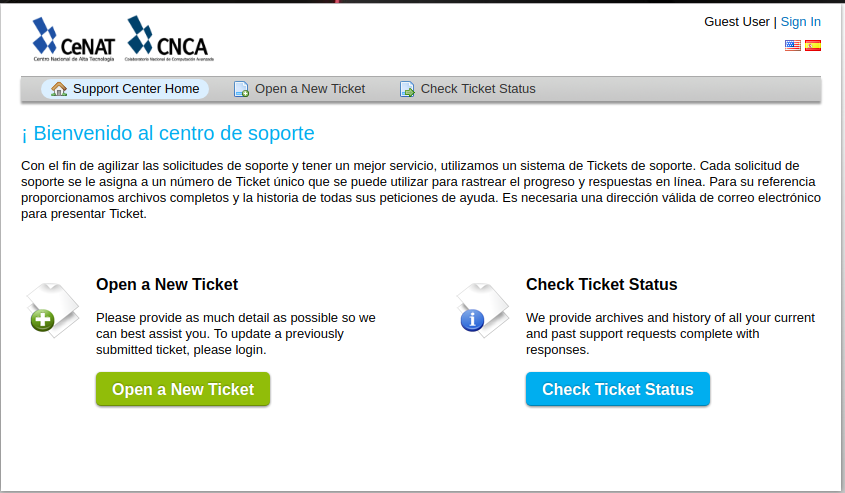
\includegraphics[width=0.5\textwidth]{osticket02.png}
\caption{Pantalla de bienvenida del sistema de tickets para soporte OSTicket.}
\label{fig:osticket:02}
\end{figure}
%%%%%%%%%%%%%%%%%%%%%%%%%%%%%%%%%%%%%%%%%%%%%%%%%%%%%%%%%%%%%%%%%%%%
Lo anterior nos lleva a la pantalla mostrada en la figura \ref{fig:osticket:03}. Desde acá, nos dirigimos donde dice \"{}I'm an agent - sign in here\"{} para iniciar sesión como adminitrador.
%%%%%%%%%%%%%%%%%%%%%%%%%%%%%%%%%%%%%%%%%%%%%%%%%%%%%%%%%%%%%%%%%%%%
\begin{figure}[H]
\centering
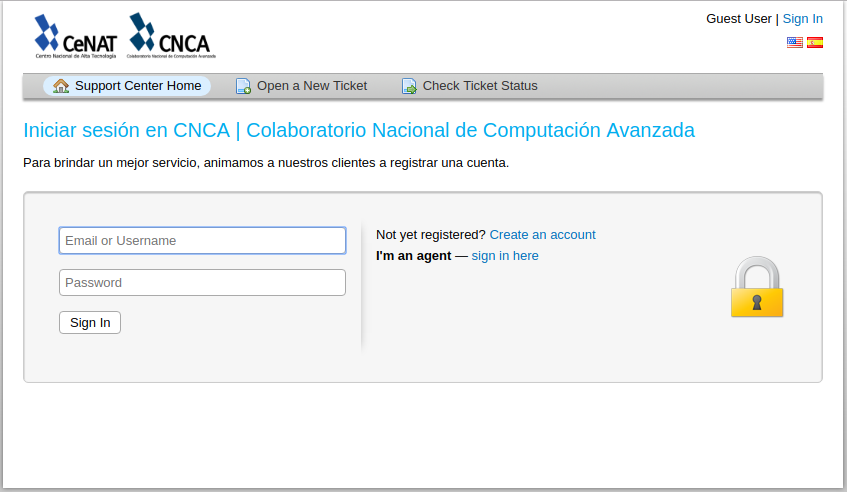
\includegraphics[width=0.5\textwidth]{osticket03.png}
\caption{Pantalla de inicio de sesión como usuario regular.}
\label{fig:osticket:03}
\end{figure}
%%%%%%%%%%%%%%%%%%%%%%%%%%%%%%%%%%%%%%%%%%%%%%%%%%%%%%%%%%%%%%%%%%%%
A partir de acá, nos lleva a la pantalla de inicio de sesión como agente del sistema de tiquetes, similar al que se muestra en la figura \ref{fig:osticket:04}. Ingresamos las credenciales e iniciamos sesión.
%%%%%%%%%%%%%%%%%%%%%%%%%%%%%%%%%%%%%%%%%%%%%%%%%%%%%%%%%%%%%%%%%%%%
\begin{figure}[H]
\centering
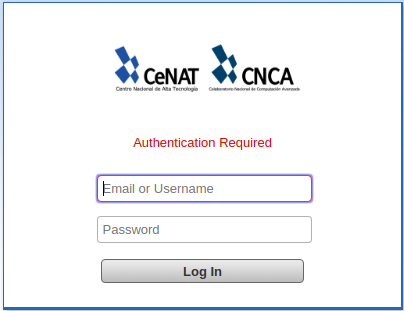
\includegraphics[width=0.5\textwidth]{osticket04.png}
\caption{Pantalla de inicio de sesión como usuario agente/administrador.}
\label{fig:osticket:04}
\end{figure}
%%%%%%%%%%%%%%%%%%%%%%%%%%%%%%%%%%%%%%%%%%%%%%%%%%%%%%%%%%%%%%%%%%%%
Esto nos dirige a la pantalla de tiquetes, según se muestra en la figura \ref{fig:osticket:05}. De acá, nos dirigimos a la esquina superior derecha y hacemos click en \"{}Agent Panel\"{}. Posteriormente nos dirigimos a la pestaña 
%%%%%%%%%%%%%%%%%%%%%%%%%%%%%%%%%%%%%%%%%%%%%%%%%%%%%%%%%%%%%%%%%%%%
\begin{figure}[H]
\centering
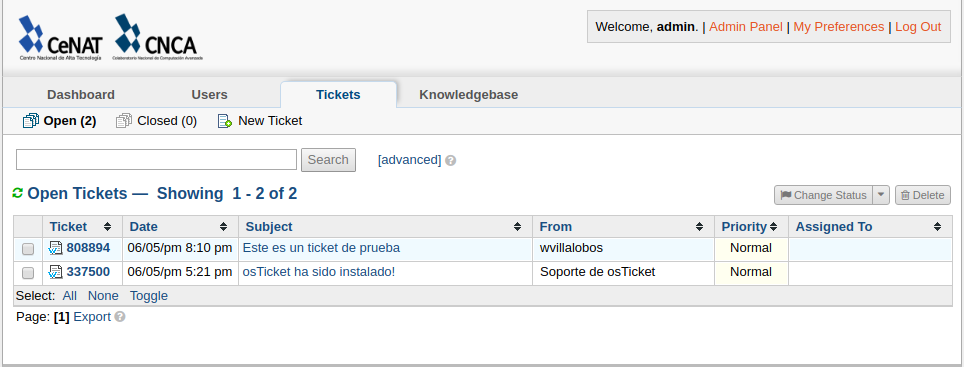
\includegraphics[width=0.5\textwidth]{osticket05.png}
\caption{Pantalla de usuario agente/administrador tras iniciar sesión.}
\label{fig:osticket:05}
\end{figure}
%%%%%%%%%%%%%%%%%%%%%%%%%%%%%%%%%%%%%%%%%%%%%%%%%%%%%%%%%%%%%%%%%%%%
Posteriormente nos dirigimos a la pestaña Access, lo cual nos dirigirá a los ajustes de acceso a los usuarios. En esta pantalla, nos aseguramos de que la configuración sea igual a la mostrada en la figura \ref{fig:osticket:00}
%%%%%%%%%%%%%%%%%%%%%%%%%%%%%%%%%%%%%%%%%%%%%%%%%%%%%%%%%%%%%%%%%%%%
\begin{figure}[H]
\centering
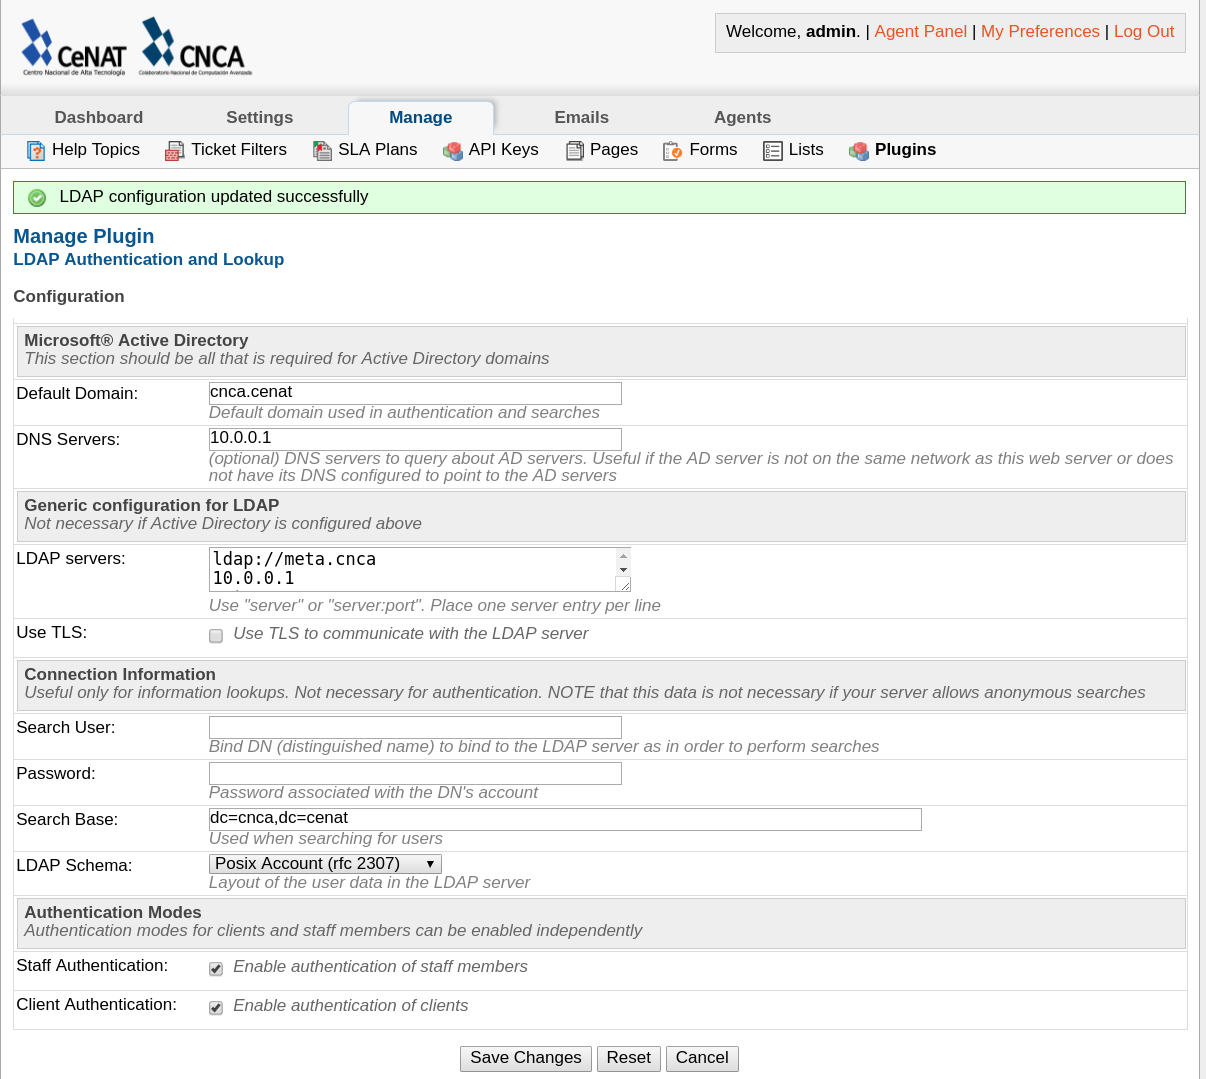
\includegraphics[width=0.5\textwidth]{osticket00.png}
\caption{Configuración del plugin para la integración del LDAP con OSTicket.}
\label{fig:osticket:00}
\end{figure}
%%%%%%%%%%%%%%%%%%%%%%%%%%%%%%%%%%%%%%%%%%%%%%%%%%%%%%%%%%%%%%%%%%%%
Finalmente, nos dirigimos a la pestaña Manage y luego a plugins, llevándonos a la pantalla mostrada en la figura \ref{fig:osticket:06}. Acá nos aseguramos que el plugin de LDAP esté instalado y habilitado, y procedemos a hacer click para realizar los ajustes necesarios.
%%%%%%%%%%%%%%%%%%%%%%%%%%%%%%%%%%%%%%%%%%%%%%%%%%%%%%%%%%%%%%%%%%%%
\begin{figure}[H]
\centering
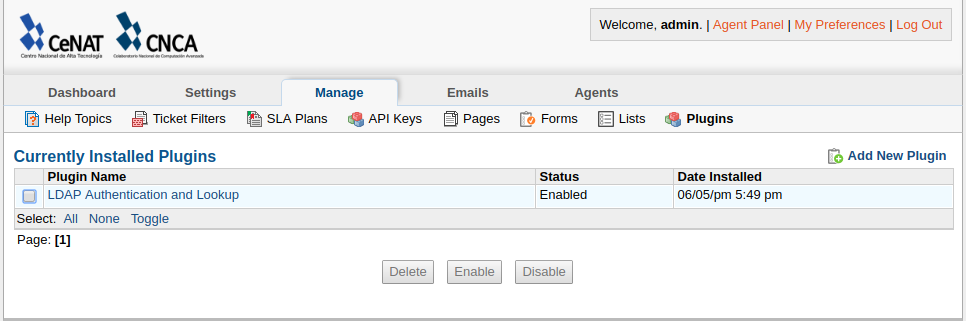
\includegraphics[width=0.5\textwidth]{osticket06.png}
\caption{Pantalla de plugins de OSTicket.}
\label{fig:osticket:06}
\end{figure}
%%%%%%%%%%%%%%%%%%%%%%%%%%%%%%%%%%%%%%%%%%%%%%%%%%%%%%%%%%%%%%%%%%%%
De acá nos dirigimos a la pantalla de ajustes del plugin de LDAP, el cual debe tener los ajustes mostrados en la figura \ref{fig:osticket:01} para que se pueda integrar corectamente el LDAP al sistema de tiquetes.
%%%%%%%%%%%%%%%%%%%%%%%%%%%%%%%%%%%%%%%%%%%%%%%%%%%%%%%%%%%%%%%%%%%%
\begin{figure}[H]
\centering
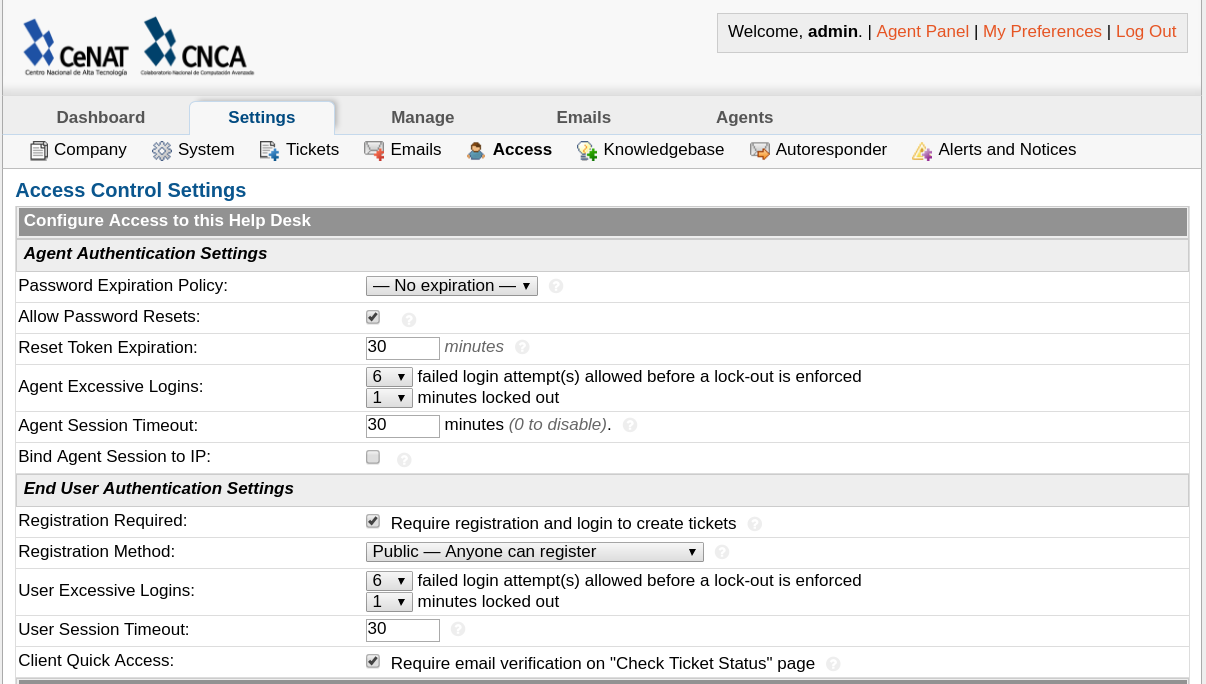
\includegraphics[width=0.5\textwidth]{osticket01.png}
\caption{Configuración de acceso para usuarios inscritos e invitados.}
\label{fig:osticket:01}
\end{figure}
%%%%%%%%%%%%%%%%%%%%%%%%%%%%%%%%%%%%%%%%%%%%%%%%%%%%%%%%%%%%%%%%%%%%
\clearpage